\documentclass[tikz,border=6pt]{standalone}
\usepackage{amsmath}
\usetikzlibrary{arrows.meta,positioning}
\begin{document}
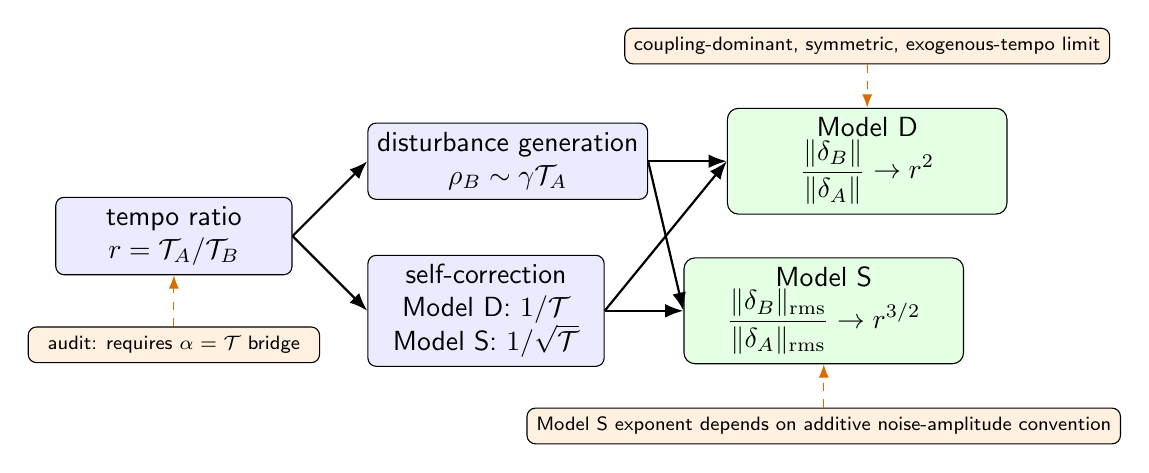
\begin{tikzpicture}[
  font=\sffamily,
  >=Latex,
  factor/.style={draw, rounded corners=3pt, fill=blue!8, align=center, minimum width=3.0cm, minimum height=0.85cm},
  result/.style={draw, rounded corners=4pt, fill=green!10, align=center, minimum width=3.55cm, minimum height=1.0cm},
  warn/.style={draw, rounded corners=3pt, fill=orange!12, align=center, font=\sffamily\scriptsize}
]

\node[factor] (tempo) {tempo ratio\\$r=\mathcal T_A/\mathcal T_B$};
\node[factor, right=0.95cm of tempo, yshift=0.95cm] (disturb) {disturbance generation\\$\rho_B \sim \gamma\mathcal T_A$};
\node[factor, right=0.95cm of tempo, yshift=-0.95cm] (correct) {self-correction\\Model D: $1/\mathcal T$\\Model S: $1/\sqrt{\mathcal T}$};

\node[result, right=1.0cm of disturb] (det) {Model D\\$\displaystyle \frac{\|\delta_B\|}{\|\delta_A\|}\to r^2$};
\node[result, right=1.0cm of correct] (stoch) {Model S\\$\displaystyle \frac{\|\delta_B\|_{\rm rms}}{\|\delta_A\|_{\rm rms}}\to r^{3/2}$};

\draw[->, thick] (tempo.east) -- (disturb.west);
\draw[->, thick] (tempo.east) -- (correct.west);
\draw[->, thick] (disturb.east) -- (det.west);
\draw[->, thick] (correct.east) -- (det.west);
\draw[->, thick] (disturb.east) -- (stoch.west);
\draw[->, thick] (correct.east) -- (stoch.west);

\node[warn, below=0.65cm of tempo, minimum width=3.7cm] (alpha)
  {audit: requires $\alpha=\mathcal T$ bridge};
\draw[->, dashed, orange!85!black] (alpha.north) -- (tempo.south);

\node[warn, above=0.55cm of det, minimum width=4.4cm] (cond)
  {coupling-dominant, symmetric, exogenous-tempo limit};
\draw[->, dashed, orange!85!black] (cond.south) -- (det.north);

\node[warn, below=0.55cm of stoch, minimum width=4.4cm] (noise)
  {Model S exponent depends on additive noise-amplitude convention};
\draw[->, dashed, orange!85!black] (noise.north) -- (stoch.south);

\end{tikzpicture}
\end{document}
